% ***********************************************************************************
% Pure LaTeX part to be inserted in a document (be careful of depencies of packages & commands)
% Prepared by XXX and YYY under the supervision of Arnaud de La Fortelle
% Fall 2017
% 12 random walk subsection of the simulation part
% ***********************************************************************************

\subgroup{4}{Yue Hu, Carlin Liao and Robert Ruigrok}

\paragraph{Model presentation}
In this example we simulate the random walk of a particle in a 2D space. A random walk is a mathematical object, known as a stochastic or random process, that describes a path that consists of a succession of random steps. In order to simulate this process, we let a particle move over a discretized grid where its motion is drawn from a set of possible directions. In this simulation we are interested in finding expected distribution of particles after a certain number of time steps as well as the position where they hit the boundaries of the spatial grid.\newline

A particle starts at a specified initial position, from where it begins moving through the grid. In our code, we used a coordinate system to represent the location of a particle as provided in figure \ref{fig:RandomWalkGrid}. The outer border of the grid is enclosed by a ``wall''. When the particle hits this wall, its motion stops and the location where it makes contact is registered.

\begin{figure}[htb]
    \label{fig:RandomWalkGrid}
	\centering
	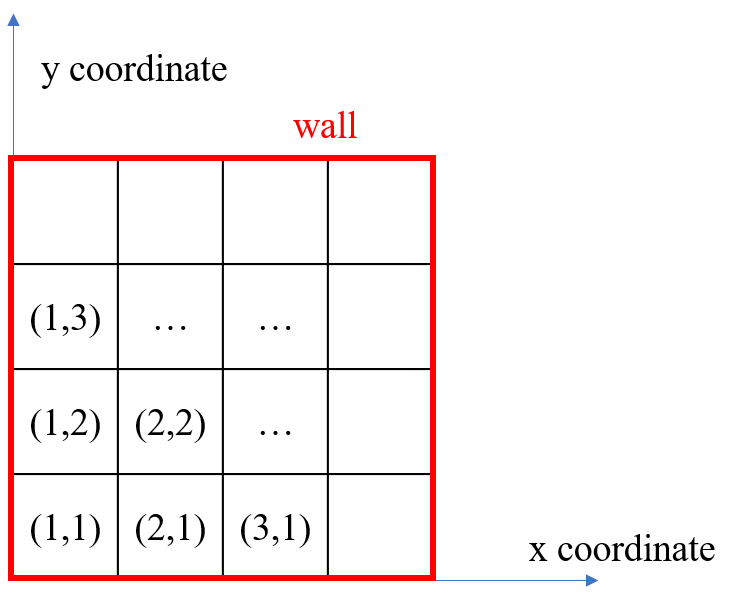
\includegraphics[width=6cm]{RandomWalkGrid.png}       
	\caption{Coordinate representation in spatial grid}
\end{figure}

The dynamics of a particle are relatively straightforward and can be described by equation \ref{eq:RandomWalkDynamics}. A particle has 5 options for its motion: moving up, right, down, left or no motion (options are depicted in figure \ref{fig:RandomWalkMotion}). Every motion has a certain probability $p$ to occur. These probabilities can be given as input and must add up to 1.

\begin{equation}
\label{eq:RandomWalkDynamics}
X_{k+1}(x,y) = X_k(x,y) +  \begin{cases}
(0,1) &\text{with probability $p\uparrow$}\\
(1,0) &\text{with probability $p\rightarrow$}\\
(0,-1) &\text{with probability $p\downarrow$}\\
(-1,0) &\text{with probability $p\leftarrow$}\\
(0,0) &\text{with probability $p\ \bullet$}
\end{cases}
\end{equation}



\begin{figure}[htb]
    \label{fig:RandomWalkMotion}
	\centering
	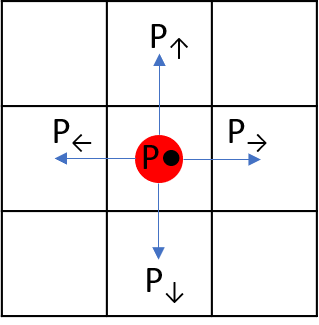
\includegraphics[width=3cm]{RandomWalkMotion.png}       
	\caption{Potential motion per time step}
\end{figure}


\paragraph{Implementation} 
At the top of the file, it is possible to set the grid size, starting position of particles, \# of particles, simulation horizon and motion direction probabilities. The script will also generate snapshots of the particle distribution at different moments in time during the simulation. By selecting the number of subplots, you can determine how many instances you would like to see. This will provide insights into how the particle distribution develops over time. \newline

Particles are simulated one at a time. The simulation runs until the time horizon $T$ is reached or the particle hits the wall. Their position is saved in a 3-dimensional array (time, x-position, y-position) at specified moments in time only; this way the amount of required memory is kept to a minimum. %You do not save the position of every particle at every time step, but you only ``count'' their positions at time steps that you are interested in. Information about individual particles gets lost, but that is fine.
\newline

Information about where particles hit the wall is included in the same arrays. This data ``circumvents'' the $n \times n$ data about the particle distribution within the grid. As a result, when we plot the full array we can see the distribution of particles in the grid at their respective location, and the distribution of particles at the wall directly ``behind'' the wall.\newline

\begin{lstlisting}[language = python, caption = 2D Ramdom Walk Simulation]
import numpy as np
import matplotlib.pyplot as plt
from random import *
import pylab

############## START INPUT #################

GridSize = 20 # will create an 20x20 square grid
Pos_init = np.ceil(np.array([0.4,0.4])*GridSize)  # start position
T = 0.3*np.power(GridSizeSquare, 2)  # total # of time steps
n_particles = 10000 # number of particles, 10000+ recommended
# specify subplots for intermediate time snap shots
subplot_row = 2             
subplot_column = 2
#define the probabilities of motion: ([up,right,down,left,0]) 
motion_prob = np.array([0.2,0.2,0.2,0.2,0.2])

############## END INPUT #################

x_grid = GridSizeSquare
y_grid = GridSizeSquare
n_subplot = subplot_row*subplot_column
# calculate time step for snapshots of process
Plot_interval = np.floor((T-1)/(n_subplot-1))
# Normalize probabilities in case they don't add up to 1
motion_prob = motion_prob/np.sum(motion_prob)
# define the change in coordinates of every motion:
motion_xy = np.array([[0,1],[1,0],[0,-1],[-1,0],[0,0],])
motion_prob_sum = np.cumsum(motion_prob)
# this is used later to draw from with randomizer

# make an empty data grid to sum the particle positions
Data = np.zeros((x_grid+2,y_grid+2))  # +2 for wall data
# Some resizing here and later are for ploting purposes
Data_resized = np.zeros((Data.shape[0]+1,Data.shape[1]+1))
# Create a new empty data set for the intermediate plots:
Data_Snap=np.zeros((n_subplot,Data_resized.shape[0],Data_resized.shape[1]))

# construct some arrays for plotting later on:
xx, yy = pylab.meshgrid(
    pylab.linspace(-1,x_grid+1,x_grid+3),
    pylab.linspace(-1,y_grid+1,y_grid+3))

# start loop over all the particles
for i in range(1, n_particles+1):
    # Initialize simulation
    t = 0
    HitWall = False
    Pos = Pos_init
    Subplot = 1
    
    # Simulation Process
    while t < T and not HitWall:
        MotionRandom = random()
        IndexMotion = np.argmax(motion_prob_sum>MotionRandom)
        Pos = Pos + motion_xy[IndexMotion,:] 
        
        # Now check for hitting the wall
        if Pos[0] == 0|x_grid+1 or Pos[1] == 0|y_grid+1:
            if Subplot <= n_subplot:             
                Data_Snap[Subplot-1,Pos[0],Pos[1]] = \
                Data_Snap[Subplot-1,Pos[0],Pos[1]]+1
            HitWall = True

        # Record the position for each time snap
        if t % Plot_interval==0 and Subplot <= n_subplot and not(HitWall):        
            Data_Snap[Subplot-1,Pos[0],Pos[1]] =\
            Data_Snap[Subplot-1,Pos[0],Pos[1]]+1
            Subplot = Subplot+1        
        
        t = t+1
    
    #Save the final results
    Data[Pos[0],Pos[1]] = Data[Pos[0],Pos[1]] + 1
    Data_resized[:-1,:-1] = Data       

# Add the particles that hit the wall in earlier time steps
# to the later plots
Data_Snap_New = np.cumsum(Data_Snap,axis=0)
Data_Snap_New[:,1:x_grid+1,1:y_grid+1] = Data_Snap[:,1:x_grid+1,1:y_grid+1]

# Visualize the outcomes at each snap of process
plt.figure()
for j in range(1, n_subplot+1):
    pylab.subplot(subplot_row, subplot_column, j)
    pylab.pcolor(xx,yy,np.transpose(Data_Snap_New[j-1,:,:]))
    Str = 'Distribution at t = ' + str((j-1)*Plot_interval+1)
    pylab.title(Str)
    # add a color bar
    pylab.colorbar()
    pylab.hold(True)
    pylab.plot([0, x_grid],[0, 0], 'r',
               [0, x_grid],[y_grid, y_grid], 'r',[0, 0],[0, y_grid], 'r',
               [x_grid, x_grid],[0, y_grid], 'r')
    pylab.plot(Pos_init[0]-0.5,Pos_init[1]-0.5,'ro')

pylab.show()

# Plot the final distribution
plt.figure()
pylab.pcolor(xx,yy,np.transpose(Data_resized))
pylab.title('Final distribution at t = %d, including hitting walls' %T)
# add a color bar 
pylab.colorbar()
pylab.hold(True)
pylab.plot([0, x_grid],[0, 0], 'r',
           [0, x_grid],[y_grid, y_grid], 'r',[0, 0],[0, y_grid], 'r',
           [x_grid, x_grid],[0, y_grid], 'r')
pylab.plot(Pos_init[0]-0.5,Pos_init[1]-0.5,'ro')
pylab.show
\end{lstlisting}



\paragraph{Results}
In this section we included two simulation for both a $10x10$ grid and a $20 \times 20$ grid, with a different simulation time horizon $T$. Both simulations use 10,000 particles and have a motion probability of $0.2$ in all directions. \newline

It is clearly visible how the particles spread out over time and make their way to the walls over time. The more particles that are simulated per grid resolution, the smoother the distribution becomes. You can clearly see that 10,000 particles simulated lead to a clean distribution in the smaller plot of figure \ref{fig:RandomWalk10}, while the larger plot of \ref{fig:RandomWalk20} shows a more grainy distribution.

\begin{figure}[htb]
    \label{fig:RandomWalk10}
	\centering
	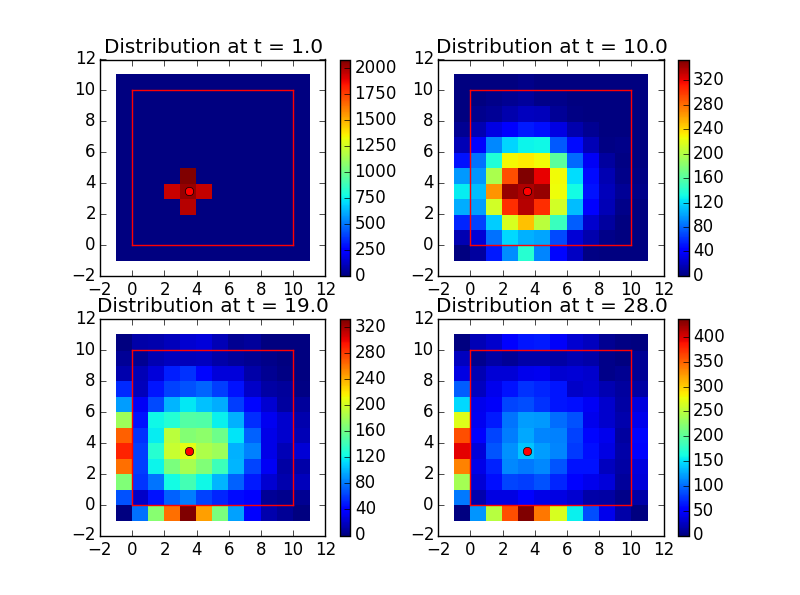
\includegraphics[width=14cm]{figure10x10.png}       
	\caption{Particle distribution for $10 \times 10$ grid at different time steps}
\end{figure}

\begin{figure}[htb]
    \label{fig:RandomWalk20}
	\centering
	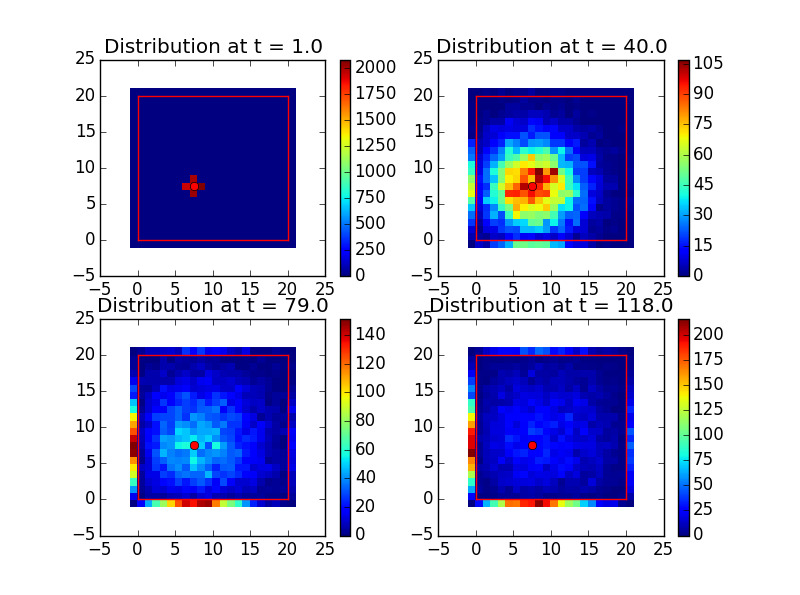
\includegraphics[width=14cm]{figure20x20.png}       
	\caption{Particle distribution for $20 \times 20$ grid at different time steps}
\end{figure}


 
\paragraph{Interpretation}
{\it Relate these quantities to the model and to theoretical knowledge of the course.}\newline

{\it I think this motion is described by Fick's Law in 2 dimension. The concentration on a specific point changes over time, depending on the concentration of its surroundings. Should we derive why the second derivative matters? $\phi$ is the concentration, $D$ the diffusion coefficient.}

\begin{equation}
\label{eq:FicksLaw}
\frac{d\phi}{dt} = D\nabla\phi = D \big(\frac{d^2\phi}{dx^2} + \frac{d^2\phi}{dy^2}\big)
\end{equation}


 \paragraph{Conclusion}
 \textit{What have we learned? Is everything aligned (theory and practice)? What was difficult? Provide perspectives.}
 
 The dynamics of the random walk were easy to model. The challenge in this simulation was to save the data for the intermediate time steps. Since the particles are simulated one by one for the full time horizon, we had to write some non-intuitive code to save the location of every particle at the relevant intermediate time steps. \newline
 
 From the lecture we recall that diffusion distance scales with the square root of time. Here we tried to simulate that. When doubling the grid size and taking a four times higher simulation horizon, the distribution looks similar. However, we have the idea that the scaling did not work for 100\%. At the end of the scaled simulation horizon, it seems as if the smaller grid has relatively more particles in the grid than the larger grid has. What could cause this difference?
 
